\subsection{OmniTransfer: Page Recall and Action Grounding}
\label{sec:eval-omnitransfer}

We evaluate the two outputs of \textsc{OmniTransfer}: a page embedding for
runtime page recall and a node-level ranking for cross-platform action
grounding.  The page-recall experiment uses the application-disjoint
PAPT-heldout-128 split, which contains 128 phone--tablet page pairs from 15
applications excluded from training.  For each source page, all target pages
from the same held-out application form the retrieval gallery.  The action
experiment uses the held-out ASE Test split with 98 page pairs, 196 mapping
directions, and 1,286 reviewed node correspondences.  Each source node is
ranked against all target XML nodes with valid bounding boxes; thus, Top-$k$
measures whether any annotated target appears among the first $k$ candidates.
The two experiments answer complementary questions.  Page recall tests whether
two device-specific observations can be recognized as the same GUI state before
an action is replayed.  Action grounding tests the subsequent local decision:
given a recorded source element and a live target page, can the system identify
the target node without reusing the source coordinate, resource identifier, or
platform-specific selector?  We therefore report the two heads separately;
page-level retrieval is not treated as evidence that an individual action has
already been grounded.

\begin{figure*}[t]
  \centering
  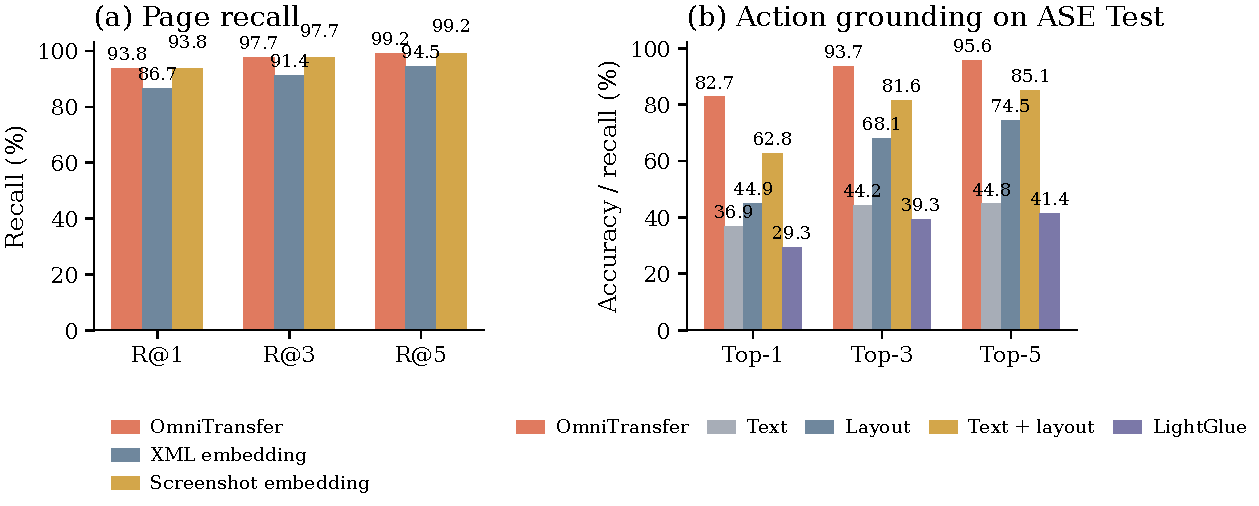
\includegraphics[width=0.72\textwidth]{figs/generated/omnitransfer_components.pdf}
  \caption{\textbf{Page recall and action grounding with \textsc{OmniTransfer}.}
  (a) Page-recall accuracy on the application-disjoint PAPT-heldout-128 split.
  (b) Action grounding on the held-out ASE Test split under the same all-node
  candidate policy.  The component ablation is reported in
  Table~\ref{tab:omnitransfer-ablation}, where each row explains the role of
  one operation in the model.  The four direct baselines use no ASE training
  labels; \textsc{OmniTransfer} is trained on the disjoint ASE training split.}
  \label{fig:omnitransfer-components}
\end{figure*}

\begin{table}[t]
  \centering
  \scriptsize
  \caption{Action-grounding results on the current ASE Test protocol.  All rows
  use the same 98 page pairs, 196 directions, and all-node candidate policy.
  LightGlue reports mean page-pair inference time, whereas the local matcher
  reports mean action-head time.}
  \label{tab:omnitransfer-components}
  \resizebox{\columnwidth}{!}{%
  \begin{tabular}{lrrrr}
    \toprule
    Method & Top-1 & Top-3 & Top-5 & Mean ms \\
    \midrule
    Text matching & 36.86 & 44.25 & 44.79 & -- \\
    Layout scaling & 44.95 & 68.12 & 74.49 & -- \\
    Text + layout (handcrafted) & 62.75 & 81.65 & 85.07 & -- \\
    \textsc{LightGlue} & 29.32 & 39.35 & 41.37 & 1185.14 \\
    \textsc{OmniTransfer}
      & \textbf{82.74} & \textbf{93.70} & \textbf{95.65} & 22.30 \\
    \bottomrule
  \end{tabular}}
\end{table}

\paragraph{Page recall.}
We construct a same-application retrieval gallery in which the query is a page
captured on one device and the candidates are pages captured on the other
device.  This isolates page identity from application recognition: a method
must use the contents and organization of the GUI rather than the application
name alone.  Screenshot embedding is a visual reference that compares rendered
appearance directly, whereas XML embedding tests whether the serialized
hierarchy is sufficient when the two platforms expose different attributes and
nesting.  The learned page head reaches 93.75\% R@1 and 99.22\% R@5, matching
the screenshot reference and showing that its compact representation retains
the page-level cues needed for retrieval.

The important observation is not only that the retrieval scores are high, but
that the evidence can be obtained from the same local GUI representation used
by the action head.  The screenshot and XML references invoke embedding models
as model-service calls; their recorded service times should not be interpreted
as the speed of a locally deployed embedding model.  The page head instead
reuses locally encoded nodes and performs a lightweight page readout, so it
avoids sending screenshots, XML, or user-visible text to a remote service.  We
therefore report the remote-deployment measurements separately: they expose
the practical boundary between an accurate server-side embedding experiment
and a page representation that can be queried continuously at runtime.

\begin{table}[t]
  \centering
  \scriptsize
  \caption{Embedding deployment feasibility on the remote \texttt{9207} server.}
  \label{tab:omnitransfer-embedding-deployment}
  \resizebox{\columnwidth}{!}{%
  \begin{tabular}{lrrrrrrr}
    \toprule
    Input & Tokens & First s & Repeat s & Dim. & Memory GB & Limit \\
    \midrule
    HTML-like XML & 369 & 18.4 & -- & 2048 & 2.7 & 2048 \\
    Screenshot & 272 & 30.8 & 0.23 & 2048 & 2.8 & 2048 \\
    \bottomrule
  \end{tabular}}
\end{table}

\paragraph{Embedding deployment boundary.}
The deployment measurements in Table~\ref{tab:omnitransfer-embedding-deployment}
were collected on the remote \texttt{9207} server and are reported separately from the
PAPT retrieval accuracy table.  They show that the evaluated embedding service
is not a direct on-device, real-time replacement for the lightweight page head:
the first embedding requires 18.4\,s for a short HTML-like input and about
30.8\,s for a screenshot, while the resident memory is 2.7--2.8\,GB.  The
apparently small screenshot token count does not imply low computation, because
visual encoding cost is not proportional to the PNG file size or token count.
HTML-like input is instead sensitive to sequence length: the reported 4\,KB
case used 1,509 tokens and exceeded 60\,s, while the 8\,KB case used 2,934
tokens and exceeded the 2,048-token context limit.  An unscaled screenshot also
exceeded 180\,s and caused memory/swap pressure; resizing the long edge to 512
pixels is therefore required for a controlled service call.  Sending a
screenshot or XML to a remote embedding service additionally exposes GUI text,
layout, and potentially user content to the server.  This establishes an
increased privacy exposure surface through transport, logging, access control,
and multi-tenant isolation; it is not evidence that a data leak has already
occurred.  The appropriate conclusion is that this embedding method may be
usable for offline or low-frequency server-side retrieval under strict data
controls, but should not be called once per frame on a mobile device.  The
local OmniTransfer page head remains the appropriate runtime path.

\paragraph{Action grounding.}
We evaluate action transfer as an all-node ranking problem, not as a lookup of
matching IDs.  Each baseline is deliberately chosen to expose a different
failure mode.  Exact normalized text matching asks whether the label alone is
enough; it covers only 51.94\% of queries and reaches 36.86\% Top-1 because a
label may be missing, duplicated, translated, or attached to a different XML
node on the other platform.  Layout scaling asks whether the source bounding
box can be transferred geometrically; it improves Top-1 to 44.95\%, but fails
when Android and iOS group the same function differently.  Combining text and
layout with a fixed handcrafted rule reaches 62.75\% Top-1 and 85.07\% R@5.
This improvement shows that the two signals are complementary, while the
remaining errors show why a fixed merge cannot decide which signal is reliable
for each widget.

We also run pretrained \textsc{LightGlue} as a conventional visual matching
reference.  It reaches 29.32\% Top-1, 39.35\% R@3, and 41.37\% R@5 with
69.83\% visual-evidence coverage, and its page-pair inference averages
1,185.14\,ms on CPU.  This result is informative because it is not a weak
version of the same model: \textsc{LightGlue} matches image keypoints, whereas
the evaluation target is an XML node with a semantic role and a bounding box.
Pooling visual matches into node boxes cannot recover missing text, hierarchy,
parent--child structure, or the fact that two visually similar controls may
represent different actions.  The gap therefore identifies a mismatch between
generic image correspondence and cross-platform GUI correspondence.

\textsc{OmniTransfer} addresses this mismatch in one ranking pipeline.  It first
forms a comparable multimodal descriptor for every source and target node,
then calibrates each descriptor with a sparse local neighborhood, and finally
scores and verifies candidate pairs.  The model can use surrounding labels,
container role, sibling order, and local geometry when the target node itself
is ambiguous, while still using visual evidence when text is absent.  This
joint treatment reaches 82.74\% Top-1, 93.70\% R@3, and 95.65\% R@5.  The
difference between Top-1 and Top-3 is itself a useful phenomenon: the model
resolves most correspondences immediately, and many remaining mistakes retain
the correct node among a small candidate set rather than confusing it with an
arbitrary page element.  The action head takes 22.30\,ms on average in the
Apple M4 model-only measurement, and the complete 1,194,582-parameter
checkpoint performs inference locally without API calls.

The ranking distribution makes this behavior concrete.  Of the 1,286 reviewed
correspondences, 1,064 are correct at Rank~1, 141 additional correspondences
are recovered at Ranks~2--3, and 25 additional correspondences are recovered
at Ranks~4--5; 56 annotated targets remain below Rank~5.  Thus, the Top-1
shortfall is not uniformly random: a substantial portion of failures is a
near-miss that can be exposed to confidence-aware execution or VLM fallback.
The residual errors are concentrated in the cases that motivate the design,
including duplicated controls, platform-specific grouping, missing text, and
large XML/layout differences.  These cases explain why page-level similarity
alone is insufficient for safe action replay.

\paragraph{Ablations.}
We conduct controlled component ablations on the same ASE Test split using a
fixed checkpoint and the same all-node candidate policy.  The purpose is not to
create additional competing methods, but to remove one source of evidence at a
time and observe which kind of ambiguity reappears.  The full configuration
obtains 82.74\% Top-1, 93.70\% Top-3, and 95.65\% Top-5; all differences below
are computed relative to this fixed configuration.

\begin{table}[t]
  \centering
  \scriptsize
  \caption{Unified component ablation on ASE Test.  All rows use the same fixed
  checkpoint, 98 page pairs, 196 mapping directions, and 1,286 reviewed
  correspondences.}
  \label{tab:omnitransfer-ablation}
  \resizebox{\columnwidth}{!}{%
  \begin{tabular}{lrrrr}
    \toprule
    Configuration & Top-1 & Top-3 & Top-5 & $\Delta$ Top-1 \\
    \midrule
    Full configuration
      & \textbf{82.74} & \textbf{93.70} & \textbf{95.65} & 0.00 \\
    Multimodal GUI element encoding only
      & 59.41 & 73.17 & 79.08 & $-23.33$ \\
    Local-context calibration without learned
    relevance-weighted aggregation
      & 75.12 & 89.11 & 93.23 & $-7.62$ \\
    Target matching and verification without
    local score refinement
      & 73.41 & 86.08 & 89.74 & $-9.33$ \\
    Multimodal GUI element encoding without visual crop
      & 74.81 & 87.87 & 92.15 & $-7.93$ \\
    \bottomrule
  \end{tabular}}
\end{table}

The ablations reveal a progression rather than four unrelated score changes.
When the graph and matching stages are removed and only multimodal GUI element
encoding remains, Top-1 falls by 23.33 percentage points.  The phenomenon is
that a node can look plausible in isolation while its role is wrong: duplicate
labels and platform-specific wrappers cannot be resolved from the node's own
attributes.  Removing learned relevance-weighted aggregation lowers Top-1 by
7.62 points.  This shows that local context is useful only when the model can
select the informative neighbors; uniformly merging parent, sibling, and
spatial information can dilute the signal instead of disambiguating it.

Removing local score refinement in target matching and verification causes a
9.33-point Top-1 drop.  A good representation therefore does not by itself
guarantee a safe action: candidate scores still need local comparison and
mutual verification to separate near-duplicate controls.  Finally, masking the
visual crop reduces Top-1 by 7.93 points, showing that visual evidence supplies
information that text and XML cannot provide for unlabeled icons or controls
whose rendered appearance is distinctive.  Taken together, the results
support the intended division of labor: multimodal encoding describes the
widget, local-context calibration explains its role, and target matching and
verification decides whether a concrete live node is safe to execute.

\paragraph{Protocol boundary.}
The current table uses the reproduced ASE Test result for \textsc{LightGlue},
not the earlier 52.26\% value from a separate 1,661-query visual-widget test.
That historical value is retained only in the authoritative experiment report
as supporting evidence because its manifest, candidate set, and Top-$k$
reporting protocol differ from ASE Test.
